%
% Main document
% ===========================================================================
% This is part of the document "Project documentation template".
% Authors: brd3, kaa1
%

%---------------------------------------------------------------------------
\documentclass[
	a4paper,					% paper format
	10pt,							% fontsize
	twoside,					% double-sided
	openright,				% begin new chapter on right side
	notitlepage,			% use no standard title page
	parskip=half,			% set paragraph skip to half of a line
]{scrreprt}					% KOMA-script report
%---------------------------------------------------------------------------

\raggedbottom
\KOMAoptions{cleardoublepage=plain}			% Add header and footer on blank pages


% Load Standard Packages:
%---------------------------------------------------------------------------
\usepackage[standard-baselineskips]{cmbright}

\usepackage[ngerman]{babel}										% german hyphenation
%\usepackage[latin1]{inputenc}  							% Unix/Linux - load extended character set (ISO 8859-1)
\usepackage[utf8]{inputenc}  							% Windows - load extended character set (ISO 8859-1)
\usepackage[T1]{fontenc}											% hyphenation of words
\usepackage{textcomp}													% additional symbols
\usepackage{ae}																% better resolution of Type1-Fonts 
\usepackage{fancyhdr}													% simple manipulation of header and footer 
\usepackage{etoolbox}													% color manipulation of header and footer
\usepackage{graphicx}                      		% integration of images
\usepackage{float}														% floating objects
\usepackage{caption}													% for captions of figures and tables
\usepackage{booktabs}													% package for nicer tables
\usepackage{tocvsec2}													% provides means of controlling the sectional numbering
%---------------------------------------------------------------------------

% Load Math Packages
%---------------------------------------------------------------------------
\usepackage{amsmath}                    	   	% various features to facilitate writing math formulas
\usepackage{amsthm}                       	 	% enhanced version of latex's newtheorem
\usepackage{amsfonts}                      		% set of miscellaneous TeX fonts that augment the standard CM
\usepackage{amssymb}													% mathematical special characters
\usepackage{exscale}													% mathematical size corresponds to textsize
%---------------------------------------------------------------------------

% Package to facilitate placement of boxes at absolute positions
%---------------------------------------------------------------------------
\usepackage[absolute]{textpos}
\setlength{\TPHorizModule}{1mm}
\setlength{\TPVertModule}{1mm}
%---------------------------------------------------------------------------					
			
% Definition of Colors
%---------------------------------------------------------------------------
\RequirePackage{color}                          % Color (not xcolor!)
\definecolor{linkblue}{rgb}{0,0,0.8}            % Standard
\definecolor{darkblue}{rgb}{0,0.08,0.45}        % Dark blue
\definecolor{bfhgrey}{rgb}{0.41,0.49,0.57}      % BFH grey
%\definecolor{linkcolor}{rgb}{0,0,0.8}     			% Blue for the web- and cd-version!
\definecolor{linkcolor}{rgb}{0,0,0}        			% Black for the print-version!
%---------------------------------------------------------------------------

% Hyperref Package (Create links in a pdf)
%---------------------------------------------------------------------------
\usepackage[
	pdftex,ngerman,bookmarks,plainpages=false,pdfpagelabels,
	backref = {false},										% No index backreference
	colorlinks = {true},                  % Color links in a PDF
	hypertexnames = {true},               % no failures "same page(i)"
	bookmarksopen = {true},               % opens the bar on the left side
	bookmarksopenlevel = {0},             % depth of opened bookmarks
	pdftitle = {Waermepumpe vs Oelbrennwertkessel},	   	% PDF-property
	pdfauthor = {brd3},        					  % PDF-property
	pdfsubject = {LaTeX Template},        % PDF-property
	linkcolor = {linkcolor},              % Color of Links
	citecolor = {linkcolor},              % Color of Cite-Links
	urlcolor = {linkcolor},               % Color of URLs
]{hyperref}
%---------------------------------------------------------------------------

% Set up page dimension
%---------------------------------------------------------------------------
\usepackage{geometry}
\geometry{
	a4paper,
	left=28mm,
	right=15mm,
	top=30mm,
	headheight=20mm,
	headsep=10mm,
	textheight=242mm,
	footskip=15mm
}
%---------------------------------------------------------------------------

% Makeindex Package
%---------------------------------------------------------------------------
\usepackage{makeidx}                         		% To produce index
\makeindex                                    	% Index-Initialisation
%---------------------------------------------------------------------------

% Glossary Package
%---------------------------------------------------------------------------
% the glossaries package uses makeindex
% if you use TeXnicCenter do the following steps:
%  - Goto "Ausgabeprofile definieren" (ctrl + F7)
%  - Select the profile "LaTeX => PDF"
%  - Add in register "Nachbearbeitung" a new "Postprozessoren" point named Glossar
%  - Select makeindex.exe in the field "Anwendung" ( ..\MiKTeX x.x\miktex\bin\makeindex.exe )
%  - Add this [ -s "%tm.ist" -t "%tm.glg" -o "%tm.gls" "%tm.glo" ] in the field "Argumente"
%
% for futher informations go to http://ewus.de/tipp-1029.html
%---------------------------------------------------------------------------
\usepackage[nonumberlist]{glossaries}
\makeglossaries

\newglossaryentry{BibTeX}{name={BibTeX},description={Programm zur Erstellung von Literaturangaben und -verzeichnissen in \TeX- oder \LaTeX-Dokumenten}}
\newglossaryentry{StwVrz}{name={Stichwortverzeichnis},description={Verzeichnis mit Stichworten aus dem Text}}



%---------------------------------------------------------------------------

% Intro:
%---------------------------------------------------------------------------
\begin{document}                              	% Start Document
\settocdepth{section}														% Set depth of toc
\pagenumbering{roman}														
%---------------------------------------------------------------------------

\providecommand{\titel}{Sole-Wasser Wärmepumpe}		%  Hier den Titel des Berichts/Thesis eingeben					% Titel der Arbeit aus Datei titel.tex lesen
\providecommand{\versionnumber}{2.0}			%  Hier die aktuelle Versionsnummer eingeben
\providecommand{\versiondate}{29.05.2016}		%  Hier das Datum der aktuellen Version eingeben				% Versionsnummer und -datum aus Datei version.tex lesen

% Set up header and footer
%---------------------------------------------------------------------------
\makeatletter
\patchcmd{\@fancyhead}{\rlap}{\color{bfhgrey}\rlap}{}{}		% new color of header
\patchcmd{\@fancyfoot}{\rlap}{\color{bfhgrey}\rlap}{}{}		% new color of footer
\makeatother

\fancyhf{}																		% clean all fields
\fancypagestyle{plain}{												% new definition of plain style	
	\fancyfoot[OR,EL]{\footnotesize \thepage} 	% footer right part --> page number
	\fancyfoot[OL,ER]{\footnotesize \titel, Version \versionnumber, \versiondate}	% footer even page left part 
}

\renewcommand{\chaptermark}[1]{\markboth{\thechapter.  #1}{}}
\renewcommand{\headrulewidth}{0pt}				% no header stripline
\renewcommand{\footrulewidth}{0pt} 				% no bottom stripline

\pagestyle{plain}
%---------------------------------------------------------------------------


% Title Page and Abstract
%---------------------------------------------------------------------------
%%
% Project documentation template
% ===========================================================================
% This is part of the document "Project documentation template".
% Authors: brd3, kaa1
%

\begin{titlepage}


% BFH-Logo absolute placed at (28,12) on A4 
% Actually not a realy satisfactory solution but working.
%---------------------------------------------------------------------------
\setlength{\unitlength}{1mm}
\begin{textblock}{20}[0,0](28,12)
	
\includegraphics[scale=1.0]{bilder/BFH_Logo_B.png}
\end{textblock}
\color{black}

% Institution / Titel / Untertitel / Autoren / Experten:
%---------------------------------------------------------------------------
\begin{flushleft}

\vspace*{21mm}

\fontsize{26pt}{40pt}\selectfont 
\titel 				\\							% Titel aus der Datei vorspann/titel.tex lesen
\vspace{2mm}

\fontsize{16pt}{24pt}\selectfont\vspace{0.3em}
Hier steht ein Untertitel 			\\							% Untertitel eingeben
\vspace{5mm}

\fontsize{10pt}{12pt}\selectfont
\textbf{Art der Arbeit (Semesterarbeit / Bachelorthesis / etc.)} \\									% eingeben
\vspace{7mm}

% Abstract (eingeben):
%---------------------------------------------------------------------------
\begin{textblock}{150}(28,100)
\fontsize{10pt}{12pt}\selectfont
[Kurztext (Abstract) einf�gen, falls gew�nscht] \\ 
Dieses Dokument dient als Vorlage f�r die Erstellung von Berichten nach den Richtlinien der BFH. Die Vorlage ist in \LaTeX{} erstellt und unterst�tzt das automatische Erstellen von diversen Verzeichnissen, Literaturangaben, Indexierung und Glossaren. Dieser kleine Text ist eine Zusammenfassung �ber das vorliegenden Dokument mit einer L�nge von 4 bis max. 8 Zeilen. \\
Das Titelbild kann in den Zeilen 157/158 der Datei template.tex ein- oder ausgeschaltet werden.
\end{textblock}

\begin{textblock}{150}(28,225)
\fontsize{10pt}{17pt}\selectfont
\begin{tabbing}
xxxxxxxxxxxxxxx\=xxxxxxxxxxxxxxxxxxxxxxxxxxxxxxxxxxxxxxxxxxxxxxx \kill
Studiengang:	\> [z.B. Elektro- und Kommunikationstechnik]	\\			% Namen eingeben
Autoren:		\> [Test Peter, M�ster R�s�]		\\					% Namen eingeben
Betreuer:	\> [Dr.~Xxxx Xxxx, Dr.~Yyyy Yyyy]		\\					% Namen eingeben
Auftraggeber:	\> [Wwwww AG]						\\					% Namen eingeben
Experten:		\> [Dr.~Zzzz Zzzz]				\\					% Namen eingeben
Datum:			\> \versiondate					\\		% aus Datei vorspann/version.tex lesen
\end{tabbing}

\end{textblock}
\end{flushleft}

\begin{textblock}{150}(28,280)
\noindent 
\color{bfhgrey}\fontsize{9pt}{10pt}\selectfont
Berner Fachhochschule | Haute �cole sp�cialis�e bernoise | Bern University of Applied Sciences
\color{black}\selectfont
\end{textblock}


\end{titlepage}

%
% ===========================================================================
% EOF
%
		% activate for Titelseite ohne Bild
%
% Project documentation template
% ===========================================================================
% This is part of the document "Project documentation template".
% Authors: brd3, kaa1
%

\begin{titlepage}


% BFH-Logo absolute placed at (28,12) on A4 and picture (16:9 or 15cm x 8.5cm)
% Actually not a realy satisfactory solution but working.
%---------------------------------------------------------------------------
\setlength{\unitlength}{1mm}
\begin{textblock}{20}[0,0](28,12)
	
\includegraphics[scale=1.0]{bilder/BFH_Logo_B.png}
\end{textblock}

\begin{textblock}{154}(28,48)
	\begin{picture}(150,2)
		\put(0,0){\color{bfhgrey}\rule{150mm}{2mm}}
	\end{picture}
\end{textblock}

\begin{textblock}{154}[0,0](28,50)
	
\includegraphics[scale=1.0]{bilder/platzhalter.jpg}			% Titelbild definieren
\end{textblock}

\begin{textblock}{154}(28,135)
	\begin{picture}(150,2)
		\put(0,0){\color{bfhgrey}\rule{150mm}{2mm}}
	\end{picture}
\end{textblock}
\color{black}

% Institution / Titel / Untertitel / Autoren / Experten:
%---------------------------------------------------------------------------
\begin{flushleft}

\vspace*{115mm}

\fontsize{26pt}{28pt}\selectfont 
\titel 				\\							% Titel aus der Datei vorspann/titel.tex lesen
\vspace{2mm}

\fontsize{16pt}{20pt}\selectfont\vspace{0.3em}
Hier steht ein Untertitel 			\\							% Untertitel eingeben
\vspace{5mm}

\fontsize{10pt}{12pt}\selectfont
\textbf{Art der Arbeit (Semesterarbeit / Bachelorthesis / etc.)} \\									% eingeben
\vspace{3mm}

% Abstract (eingeben):
%---------------------------------------------------------------------------
\begin{textblock}{150}(28,190)
\fontsize{10pt}{12pt}\selectfont
[Kurztext (Abstract) einf�gen, falls gew�nscht] \\ 
Dieses Dokument dient als Vorlage f�r die Erstellung von Berichten nach den Richtlinien der BFH. Die Vorlage ist in \LaTeX{} erstellt und unterst�tzt das automatische Erstellen von diversen Verzeichnissen, Literaturangaben, Indexierung und Glossaren. Dieser kleine Text ist eine Zusammenfassung �ber das vorliegenden Dokument mit einer L�nge von 4 bis max. 8 Zeilen. \\
Das Titelbild kann in den Zeilen 157/158 der Datei template.tex ein- oder ausgeschaltet werden.
\end{textblock}

\begin{textblock}{150}(28,225)
\fontsize{10pt}{17pt}\selectfont
\begin{tabbing}
xxxxxxxxxxxxxxx\=xxxxxxxxxxxxxxxxxxxxxxxxxxxxxxxxxxxxxxxxxxxxxxx \kill
Studiengang:	\> [z.B.Elektro- und Kommunikationstechnik]	\\			% Namen eingeben
Autoren:		\> [Test Peter, M�ster R�s�]		\\					% Namen eingeben
Betreuer:	\> [Dr.~Xxxx Xxxx, Dr.~Yyyy Yyyy]		\\					% Namen eingeben
Auftraggeber:	\> [Wwwww AG]						\\					% Namen eingeben
Experten:		\> [Dr.~Zzzz Zzzz]				\\					% Namen eingeben
Datum:			\> \versiondate					\\		% aus Datei vorspann/version.tex lesen
\end{tabbing}

\end{textblock}
\end{flushleft}

\begin{textblock}{150}(28,280)
\noindent 
\color{bfhgrey}\fontsize{9pt}{10pt}\selectfont
Berner Fachhochschule | Haute �cole sp�cialis�e bernoise | Bern University of Applied Sciences
\color{black}\selectfont
\end{textblock}


\end{titlepage}

%
% ===========================================================================
% EOF
%
			% activate for Titelseite mit Bild
%% Versionenkontrolle :
% -----------------------------------------------

\begin{textblock}{180}(15,150)
\color{black}
\begin{huge}
Versionen
\end{huge}
\vspace{10mm}

\fontsize{10pt}{18pt}\selectfont
\begin{tabbing}
xxxxxxxxxxx\=xxxxxxxxxxxxxxx\=xxxxxxxxxxxxxx\=xxxxxxxxxxxxxxxxxxxxxxxxxxxxxxxxxxxxxxxxxxxxxxx \kill
Version	\> Datum	\> Status		\> Bemerkungen		\\
0.1	\> 01.08.2013	\> Entwurf		\> Lorem ipsum dolor sit amet	\\	
0.2	\> 21.08.2013	\> Entwurf		\> Phasellus scelerisque	\\ 
0.3	\> 02.09.2013	\> Entwurf		\> Donec eget aliquam urna. Lorem ipsum dolor sit amet	\\ 
1.0	\> 12.09.2013	\> Definitiv	\> Lorem ipsum dolor sit ametPhasellus scelerisque, leo sed iaculis ornare 	\\ 
1.1	\> 04.11.2013	\> Korrektur	\> Layout angepasst	\\
1.2	\> 01.02.2014	\> Ergänzung	\> Kapitel 1.1 erweitert	\\
\end{tabbing}

\end{textblock}

\cleardoubleemptypage
\setcounter{page}{1}
\cleardoublepage
\phantomsection 
\addcontentsline{toc}{chapter}{Management Summary}
\chapter*{Zusammenfassung}
\label{chap:zusammenfassung}

Im Rahmen des Moduls \glqq Nachhaltigkeit in den Ingenieurswissenschaften\grqq{} haben wir zum Thema Wärmepumpe eine Nachhaltigkeitsanalyse des Energieverbrauchs erstellt. Dabei liegt der Fokus auf der Erdwärmepumpe, welche mit einem Erdwärmekreislauf Wärme aus bis zu 30-50 Meter Tiefe holt.

Dieses System wurde zum Vergleich einem Ölbrennwertkessel gegenübergestellt und in verschiedenen Kriterien bewertet. Für beide Systeme haben wir eine SWOT-Analyse, eine Nachhaltigkeitsrosette und eine Energiebilanz für den Betrieb erstellt.

Wir haben dafür zwei verschiedene Heizsysteme des Anbieters Junkers ausgewählt.
Zum einen die Sole-Wasser Erdwärmepumpe \glqq STM 100-1\grqq{} als aktuelle Technologie.
Und als Vergleichsystem und bisherige Technologie den Ölbrennwertkessel \glqq KUB 19-4\grqq{}.

Mit einer SWOT-Analyse betrachten wir als erstes die qualitativen Stärken und
Schwächen der beiden Systeme. Wobei hier schon einige Nachteile der Ölheizung
deutlich werden.

Danach können wir mithilfe der Nachhaltikeitsrosette die qualitativen Merkmale
der beiden Systeme subjektiv erfassen und direkt miteinander vergleichen.
Wir sehen wo die Wärmepumpe gegenüber der Ölheizung noch Aufholbedarf hat.

Zum Schluss erstellen wir für beide Systeme eine Energiebilanz.
Wir betrachten den Energieverbrauch während eines Betriebsjahres und den
damit einhergehenden Ausstoss von Treibhausgasen.

Das ganze Mini-Projekt wird abgeschlossen mit einer Schlussfolgerung und einer persönlichen Reflexion.




\cleardoubleemptypage
%---------------------------------------------------------------------------

% Table of contents
%---------------------------------------------------------------------------
\tableofcontents
\cleardoublepage
%---------------------------------------------------------------------------

% Main part:
%---------------------------------------------------------------------------
\pagenumbering{arabic}

\chapter{Einleitung}
\label{chap:einleitung}

In diesem Projekt untersuchen wir anhand zwei Heizungsmodellen von Junkers\footnote{\url{http://www.junkers.com/}} die Nachhaltigkeit einer Solewasserwärmepumpe. \\
Als Referenz für die Wärmepumpe nehmen wir die STM 100-1\footnote{\url{http://www.junkers.com/endkunde/produkte/produktinformation/produktkatalog_4416}}. Für den Ölbrennwertkessel benutzen wir den TODO.

Wir werden die Nachhaltigkeit dieser zwei Systeme untersuchen und aufzeigen was alles für den Betrieb notwendig ist. Jedoch können wir die Herstellung und Montage der Heizungen nicht miteinbeziehen, da dies nicht im Rahmen dieses Projekts machbar ist.




\chapter{SWOT Analyse}
\label{chap:swot}

\section{Wärmepumpe}


\begin{table}[h!]
\begin{tabular}[c]{|p{0.5 \textwidth}|p{0.5 \textwidth}|}
  \hline
  \textbf{Strengths} &
  \textbf{Weaknesses} \\ \hline
  
  \begin{itemize}
    \item Geringe Schadstoffemissionen
    \item Keine direkten fossilen Ressourcen
    \item Geringe Betriebskosten
  \end{itemize}
  &
  
  \begin{itemize}
    \item Montagekosten, Bohrungen
    \item Geringe Vorlauftemperatur
    \item Gute Isolierung benötigt
  \end{itemize}
  \\ \hline
  
  \textbf{Opportunities} &
  \textbf{Threats} \\ \hline
  
  \begin{itemize}
    \item Solarstrom
    \item Neubauten
    \item Hohe Effizienz
  \end{itemize}
  &
  
  \begin{itemize}
    \item Tiefer Ölpreis
    \item Strompreis
    \item Neue Heizungstechniken
  \end{itemize}  
  \\ \hline
\end{tabular}
\label{swot:warmepumpe}
\caption{SWOT Analyse einer Erdwärmepumpe}
\end{table}

\subsection{Erklärungen}

Durch den Erdwärmekreislauf benötigt die Wärmepumpe für den Betrieb wenig Energie. Auch werden dadurch keine Schadstoffe während des Betriebs freigesetzt und keine fossilen Ressourcen wie z.B Öl gebraucht.

Diese Vorteile sind aber mit gewissen Kosten verbunden. Die Montage ist sehr aufwändig und nicht Überall möglich, da ziemlich tiefe Bohrungen durchgeführt werden müssen. Auch sind Wä
rmepumpen erst wirklich effizient, wenn das Haus eine Fussbodenheizung besitzt. Dies hängt mit der eher niedrigen Vorlauftemperatur der Wärmepumpen zusammen.

In Zukunft können die Wärmepumpen sicher noch an Effizienz gewinnen. In Verbindung mit Solarzellen kann ein autonomes Heizungssystem entwickelt werden.

Die Wärmepumpe benötigt vor allem Strom für den Betrieb. Dadurch sind die Betriebskosten sehr abhängig vom Strompreis. 

\newpage

\section{Ölheizung}

\begin{table}[h!]
\begin{tabular}[c]{|p{0.5 \textwidth}|p{0.5 \textwidth}|}
  \hline
  \textbf{Strengths} &
  \textbf{Weaknesses} \\ \hline
  
  \begin{itemize}
    \item Variable Vorlauftemperaturen
    \item Einfache Montage
  \end{itemize}
  &
  
  \begin{itemize}
    \item Verbrauch fossiler Brennstoffe
    \item Schadstoffemisionen
    \item Hoher Energieverbrauch
  \end{itemize}
  \\ \hline
  
  \textbf{Opportunities} &
  \textbf{Threats} \\ \hline
  
  \begin{itemize}
    \item Tiefer Ölpreis
    \item Bessere Energieeffizienz durch neue Technologien
  \end{itemize}
  &
  
  \begin{itemize}
  	\item Ölvorkommen erschöpft
    \item Solarkraft
    \item Neue Technologien
  \end{itemize}  
  \\ \hline
\end{tabular}
\label{swot:warmepumpe}
\caption{SWOT Analyse einer Ölheizung}
\end{table}

\subsection{Erklärungen}

Ölheizungen können mit sehr hohen und variablen Vorlaufstemperaturen betrieben werden. Dadurch eignen sie sich auch für ältere Gebäude. 
Auch die Montage ist der Heizung ist eher einfach. Es wird lediglich genügend Platz für den Öltank benötigt.

Der grösste Nachteil ist ganz klar der Verbrauch von Öl und der Ausstoss von Schadstoffen. Zusätzlich wird die ganze Heizleistung aus der Ölverbrennung gewonnen.
Dadurch sind die Betriebskosten sind stark abhängig von dem Ölpreis.
Die Heizung ist aber eher ein Auslaufmodell, da nicht unendlich Öl auf der Erde zur Verfügung steht.

Durch neue Technologien wie der Wärmepumpe oder der Solarwärme, wird die Ölheizung langsam verdrängt werden. Spätestens dann, wenn das Öl knapp wird und im Preis steigt.



\chapter{Nachhaltigkeits Rosette}
\label{chap:rosette}

Für beide Systeme wird nun eine Nachhaltigkeitsrosette erstellt. Dabei besteht die Rosette aus drei Kategorien mit je vier Kriterien. Die Kategorien setzen sich zusammen aus Umwelt, Wirtschaft und Gesellschaft. Die Einteilung der Kriterien ist subjektiv, genauso wie die Bewertung der einzelnen.



\section{Bewertung}

\begin{figure}[h]
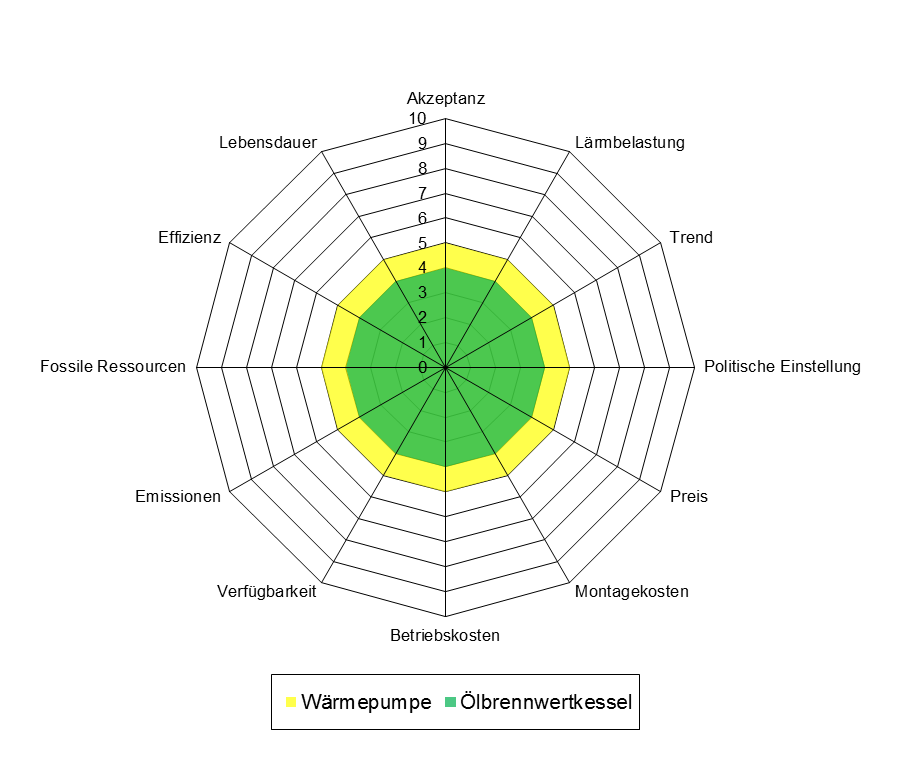
\includegraphics[scale=0.54]{bilder/Rosette.png}
\caption{Nachhaltigkeitsrosette}
\end{figure}

\begin{table}
\begin{center}
\begin{tabular}[c]{|p{0.25 \textwidth}|p{0.25 \textwidth}|p{0.25 \textwidth}|}

  \hline
  \textbf{Kriterium} &
  \textbf{Wärmepumpe} &
  \textbf{Ölbrennwertkessel} \\ \hline

  \multicolumn{3}{|c|}{\textbf{Umwelt}} \\ \hline
  
  Emissionen
  & 9 & 2 \\
  Fossile Ressourcen
  & 7 & 1 \\
  Effizienz
  & 8 & 7 \\
  Lebensdauer
  & 5 & 8 \\
  \hline
  
  \multicolumn{3}{|c|}{\textbf{Wirtschaft}} \\ \hline
  
  Preis
  & 4 & 8 \\
  Montagekosten
  & 4 & 7 \\
  Betriebskosten
  & 8 & 5 \\
  Verfügbarkeit
  & 5 & 8 \\
  \hline

  \multicolumn{3}{|c|}{\textbf{Gesellschaft}} \\ \hline

  Akzeptanz
  & 8 & 3 \\
  Lärmbelastung
  & 5 & 6 \\
  Trend
  & 7 & 4 \\
  Politische Einstellung
  & 7 & 3 \\
  \hline

\end{tabular}
\end{center}
\caption{Kriterien für Nachhaltigkeitsrosette}
\end{table}

\subsection{Erklärungen}

\begin{itemize}

\item \textbf{Emissionen}: Wärmepumpe klar im Vorteil, da so gut wie keine Emissionen. Keine Maximalwertung da bei der Stromerzeugung Emissionen entstehen können.

\item \textbf{Fossile Ressourcen}: Wärmepumpe klar vorne, da die Ölheizung von ihrem Funktionsprinzip her vollständig auf fossile Ressourcen angewiesen ist.

\item \textbf{Effizienz}: Beide ziemlich ähnlich. Ölheizungen erreichen einen Wirkungsgrad von bis zu 97\%. Die Wärmepumpe braucht viel Strom, kann aber einen Grossteil der Wärme aus dem Erdkreislauf bekommen.

\item \textbf{Lebensdauer}: Wärmepumpen haben eine Lebensdauer von 15-20 Jahren \cite{fws:faq}. Bei den Ölbrennwertkesseln rechnet man mit 20-25 Jahren\cite{offerten24:oel}.

\item \textbf{Preis}: Für eine Ölheizung muss mit etwa 15'000 CHF{offerten24:oel} gerechnet werden. Bei einer Wärmepumpe betragen die Installationskosten etwa 35'000 CHF.{offerten24:wp}

\item \textbf{Montagekosten}: Ölheizung im Vorteil, da die Wärmepumpe aufwändige Bohrungen benötigt.

\item \textbf{Betriebskosten}: Wärmepumpe hat den Vorteil des Erdwärmekreislaufs. Dadurch muss nicht die ganze Wärmeleistung von aussen zugeführt werden, wie bei der Ölheizung.

\item \textbf{Verfügbarkeit}: Ölheizung benötigt nur ein Tank, welcher fast überall platziert werden kann. Die Wärmepumpe kann nicht überall eingesetzt werden, da tiefe Bohrungen notwendig sind, welche am Standort bewilligt werden müssen. 

\item \textbf{Akzeptanz}: Durch die Globalisierung wird die Nachhaltigkeit immer mehr betont. Dadurch ist die Akzeptanz für Wärmepumpen sicher um einiges höher, da Öl schnell mit Umweltverschmutzung in Verbindung gebracht wird.

\item \textbf{Lärmbelastung}: Die Sole-Wasser Wärmepumpe ist ein bisschen lauter, wegen dem Kompressor. 

\item \textbf{Trend}: Ähnlich wie bei der Akzeptanz, begünstigen die Medien und die aktuelle Ressourcenlage den Trend nach nachhaltigeren Produkten und Systemen.

\item \textbf{Politische Einstellung}: Durch die Debatte des Atomausstiegs, wurde auch die Politik auf das Thema der Nachhaltigkeit aufmerksam. Dadurch sind Wärmepumpen sicher im Vorteil.

\end{itemize}

\chapter{Systemgrenze}
\label{chap:Systemgrenze}

Die Definition einer Systemgrenze dient dazu das System auf die Wesentlichen
Punkte zu reduzieren die untersucht werden sollen und die Analyse in einem
�berschaubaren Rahmen zuhalten.
Dazu m�ssen Annahmen getroffen werden und Vereinfachungen gemacht werden.
Die Aussagekraft des Resultates h�ngt stark damit zusammen wie diese getroffen
werden. Darum ist es besser ein m�glichst konkretes System anzuschauen anstatt
einen Allgemeinen Fall zu formulieren.

Unser Modell besteht aus einem System, in das Ressourcen eingef�hrt werden
(Input) und das daraus eine Nutzeinheit produziert, die aus dem System gewonnen
wird (Output).

\section{das System}

Wir betrachten in unserer Arbeit ein Heizsystem in Form einer
Solewasserw�rhmepumpe und als Vergleichssystem eine Heizung mit
�lbrennwertkessel.

\section{Input}

Wir betrachten in unserer Arbeit den laufenden Energieverbrauch der beiden
Systeme pro Jahr.
Beiden Systemen muss von aussen Energie zugef�gt werden um sie zu betreiben.
Daher k�nnen wir die Input Einheit in kWH ausdr�cken.

Die Solewasserw�rmepumpe bezieht ihre Energie haupts�chlich aus Zwei quellen,
der aus der Erde in Form von Erdw�rme und vom Stromnetz, vor allem um den
Kompressor zu betreiben und den Solewasserkreislauf in Gang zuhalten.
F�r uns ist vor allem der Stromverbrauch interessant, da dies ein Kostenpunkt
ist und damit auch Umweltbelastungen verbunden sind.
Als Grundlage nehmen wir den Schweizer Energiemix nach ...
Wir betrachten die Erdw�rme als �ffentlichesgut, das unbegrenzt und kostenlos
zur Verf�gung steht.

Ein �lbrennwertkessel bezieht seine Energie in Form von Heitz�l.
Wir k�nnen den Energieinput dadurch berechnen indem wir den Liter verbrauch
ansehen und die Energiedichte eines Liter �ls somit haben wir wider den
Energieinput in kWH pro Jahr erfasst.
F�r einen Liter Heiz�l dieses Typs wird so und so viel Energie gerechnet ...

Die Graueenergie, die bei der Herstellung und bei der Montage der Systeme
verbraucht wird nicht weiter in die Rechnung aufgenommen.
Wir nehmen an, das die Systeme im Wesentlich aus den gleichen Materialien
gefertigt sind und das  das Bohren der L�cher f�r die Erdw�rmegewinnung
nicht sehr ins Gewicht fallen wird.
Wir nehmen auch an, das das System f�r eine Lange Dauer erhalten bleibt.
Die Lebensdauer einer Heizung ist etwa die selbe wie die des Hauses, 
30 - 50 Jahre.
Da wir den Verbrauch pro Jahr berechnen w�rde sich die Graueenergie auf diesen
Zeitraum verteilen.

\section{Output}

Als Output haben wir die Nutzbare Heizleistung.
Um was handelt es sich hierbei?
bla bla ...

Eine Heizung ist ein Wasserkreislauf der mit einer bestimmten Temperatur
(R�cklauftemperatur) in das System eintritt und auf ein gewisses Temperaturniveau
gehoben wird (Vorlauftemperatur). Das erhitzte Wasser verl�sst das System und
gibt die aufgenommene Energie an die Umgebung ab.
 
Moderne Heizungsysteme werden als Fussbodenheizung realisiert.
Wir k�nnen die Ben�tigte Heizleistung f�r eine Fl�che von 100 $m^2$
berechnen.
berechnung wie Hier ...

Aus der Outputenergie k�nnen wir �ber den Wirkungsgrad R�ckschl�sse �ber
den Input anstellen.











\chapter{Energiebilanz}
\label{chap:bilanz}

Wir werden die Benötigte Energie und damit den $CO_2$ Ausstoss der Beiden
Heizungen Anhand der von uns festgelegten Heizleistung von 10 kW.

\section{Wärmepumpe}

Mit Hilfe des COP berechnen wir die Benötigte Stromleistung bei einer
Aussentemperatur von 6.6 C°.
Das Ergibt eine Stromleistung 1.95 kW.

Wir Errechnen anhand des vorher definierten Energiemixes den Gesammtverbrauch
der Energie um diesen Strom bereitzustellen und den damit einhergehenden $CO_2$
Ausstoss.
Wir erhalten 5.46 kW Gesammtverbrauch und 445.5 g $C0_2$.

\section{Ölbrennwertkessel}

Wir betrachten den Wirkungsgrad der Ölheizung.
Laut Herstellerangaben Liegt dieser bei 97\%.
Damit kommen wir auf einen Bedarf von 10.3 kW.
Nun beziehen wir noch die Produktionsenergie für das ÖL mit ein und erhalten
insgesammt 33.99 kW.
Der $CO_2$ Ausstoss liegt bei 290 g CO2 pro kwh.
[http://www.co2-emissionen-vergleichen.de/Heizungsvergleich/CO2-Vergleich-Heizung.html].
das Ergibt uns einen $CO_2$ Ausstoss von 9857 g.

\section{Vergleich}



\chapter{Fazit}
\label{chap:fazit}


\chapter{Persönliche Reflexion}
\label{chap:reflexion}

\subsection{Stefan Andonie}

TODO: Nur von deiner Sicht aus beschreiben

Das Miniprojekt hat uns einen Einblick gegeben in die Methoden und Begriffe
der Nachhaltigkeit.
Im Umfang des Moduls Nachhaltigkeit in den Ingenieurwissenschaften haben wir
einiges Neues gelernt und konnten eine einige interessante Aspekte anhand
des Beispiels von Heizungssystemen genauer betrachten.
Für uns Informatiker war es spannend ein solches System zu betrachten, da wir
ansonsten eher mit Virtuellen Gütern umgehen.
Wir waren uns daher zum Teil nicht so sicher wie wir die verschiedenen Methoden
anwenden sollen, zumal die Heizungsbranche ihr eigene Fachsprache hat.
Bei der Energiebilanz haben wir mehrfach das Vorgehen gewechselt.
Zum Schluss hat es uns vor allem geholfen das System einzugrenzen und zu
vereinfachen.
Rückblickend können wir festhalten, dass es mithilfe der verschiedenen Methoden
gelungen ist, eine einigermassen Zutreffende Aussage zu machen.

\subsection{Pascal Grüter}

Ich habe bei mir zuhause eine Erdwärmepumpe und es interessierte mich, ob diese Art Heizungssystem überhaupt nachhaltig ist. Durch diese Arbeit habe ich mehr erfahren über die Deklaration von Heizungen, ihrer Funktionsweise und der Nachhaltigkeit von Ölheizungen und Wärmepumpen.

Wie ich am Anfang vermutet habe, ist die Wärmepumpe um einiges nachhaltiger als eine Ölheizung. Das ist natürlich vor allem wegen dem verwendeten Öl. Die Effizienz ist auch bei Ölheizungen sehr gut, was mich erstaunt hat.

Durch diese Arbeit habe ich auch einen Einblick in die Aspekte der Nachhaltigkeit bekommen und gemerkt, dass eine vollständige Nachhaltigkeitsbewertung eines Produktes sehr komplex und aufwändig werden kann.
In Zukunft werde ich noch mehr auf die Nachhaltigkeit von Produkten und Prozessen achten als vorher und auch kritischer damit umgehen.


%---------------------------------------------------------------------------

% Selbst$ndigkeitserklärung
%---------------------------------------------------------------------------
%\cleardoublepage
%\phantomsection 
%\addcontentsline{toc}{chapter}{Selbständigkeitserklärung}
%\chapter*{Selbst�ndigkeitserkl�rung}
\label{chap:selbstaendigkeitserklaerung}

\vspace*{10mm} 

Ich/wir best�tige/n, dass ich/wir die vorliegende Arbeit selbstst�ndig und ohne Benutzung anderer als der im Literaturverzeichnis angegebenen Quellen und Hilfsmittel angefertigt habe/n. S�mtliche Textstellen, die nicht von mir/uns stammen, sind als Zitate gekennzeichnet und mit dem genauen Hinweis auf ihre Herkunft versehen. 

\vspace{15mm}

\begin{tabbing}
xxxxxxxxxxxxxxxxxxxxxxxxx\=xxxxxxxxxxxxxxxxxxxxxxxxxxxxxx\=xxxxxxxxxxxxxxxxxxxxxxxxxxxxxx\kill
Ort, Datum:		\> [Biel/Burgdorf], \versiondate \\ \\ 
Namen Vornamen:	\> [Test Peter] 	\> [M�ster R�s�] \\ \\ \\ \\ 
Unterschriften:	\> ......................................\> ...................................... \\
\end{tabbing}

%---------------------------------------------------------------------------

% Glossary
%---------------------------------------------------------------------------
\cleardoublepage
\phantomsection 
\addcontentsline{toc}{chapter}{Glossar}
\renewcommand{\glossaryname}{Glossar}
\printglossary
%---------------------------------------------------------------------------

% Bibliography
%---------------------------------------------------------------------------
\cleardoublepage
\phantomsection 
\addcontentsline{toc}{chapter}{Literaturverzeichnis}
\bibliographystyle{IEEEtranS}
\bibliography{datenbanken/bibliography}{}
%---------------------------------------------------------------------------

% Listings
%---------------------------------------------------------------------------
\cleardoublepage
\phantomsection 
\addcontentsline{toc}{chapter}{Abbildungsverzeichnis}
\listoffigures
\cleardoublepage
\phantomsection 
\addcontentsline{toc}{chapter}{Tabellenverzeichnis}
\listoftables
%---------------------------------------------------------------------------

% Index
%---------------------------------------------------------------------------
%\cleardoublepage
%\phantomsection 
%\addcontentsline{toc}{chapter}{Stichwortverzeichnis}
%\renewcommand{\indexname}{Stichwortverzeichnis}
%\printindex
%---------------------------------------------------------------------------

% Attachment:
%---------------------------------------------------------------------------
\appendix
\settocdepth{section}
%\chapter{Beliebiger Anhang}
\label{chap:bel_anhang}

Phasellus eget velit massa, sed faucibus nisi. Etiam tincidunt libero viverra lorem bibendum ut rutrum nisi volutpat. Donec non quam vitae lacus egestas suscipit at eu nisi. Maecenas non orci risus, at egestas tellus. Vivamus quis est pretium mauris fermentum consectetur. Cras non dolor vitae nulla molestie facilisis. Aliquam euismod nisl eget risus pretium non suscipit nulla feugiat. Nam in tortor sapien. Nam lectus nibh, laoreet eu ultrices nec, consequat nec sem. Nulla leo turpis, suscipit in vulputate a, dapibus molestie quam. Vestibulum pretium, purus sed suscipit tempus, turpis purus fermentum diam, id cursus enim mi a tortor. Proin imperdiet varius pellentesque. Nam congue, enim sit amet iaculis venenatis, dui neque ornare purus, laoreet porttitor nunc justo vel velit. Suspendisse potenti. Nulla facilisi.

%---------------------------------------------------------------------------

%---------------------------------------------------------------------------
\end{document}

